\subsection{Game}

\subsubsection{Introduction}
The game we have implemented is {\it The Scorched Land Defense} as described in the compendium. The game lets
two players play concurrently. Player A is a Tank starting in the lower left corner. The tanks
mission is to get to the upper right corner before it gets shot by the cannon. The cannon is
controlled by Player B. Its objective is to shoot the tank before it reaches its corner. The cannon
can use the Scorched land defence tactic by blowing up land in the field. The tank cannot drive
where the cannon has made a shot, because the field is on fire.\\
\\
Each player has 4 lifes and the game ends when one player has been defeated 4 times

\subsubsection{How to play}
\begin{figure}[h]
  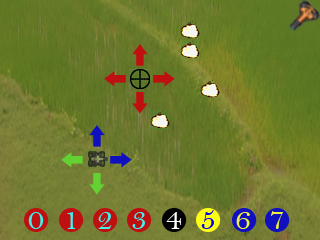
\includegraphics[width=350px]{graphics/buttons_illustration.jpg}
  \caption{Screen shot from game with controls}
\end{figure}
Note: The button numbering is reverse on the development board.\\
\\
Player A uses button 5-7 and Player B has buttons 0-4. Player A has two modes which it uses button 5
to toggle between. It can use buttons 6 and 7 to either move North and East or South and West.\\
\\
Player B uses button 0, 1, 2 and 3 to move its aim left, down, up and right. It shots it cannon on
the field where its aiming currently with button 4.
\newpage
\subsubsection{Design}

The /game folder contains the objects that is used in the game. The most important is the {\bf Controller}
which handles the communication between the different modules in the game. The {\bf Cannon}, {\bf Tank} and
{\bf Field} are models for the objects in the game. The {\bf Button} and {\bf Led} objects are
wrappers around the character device drivers, to make communication easier.

\begin{figure}[h]
  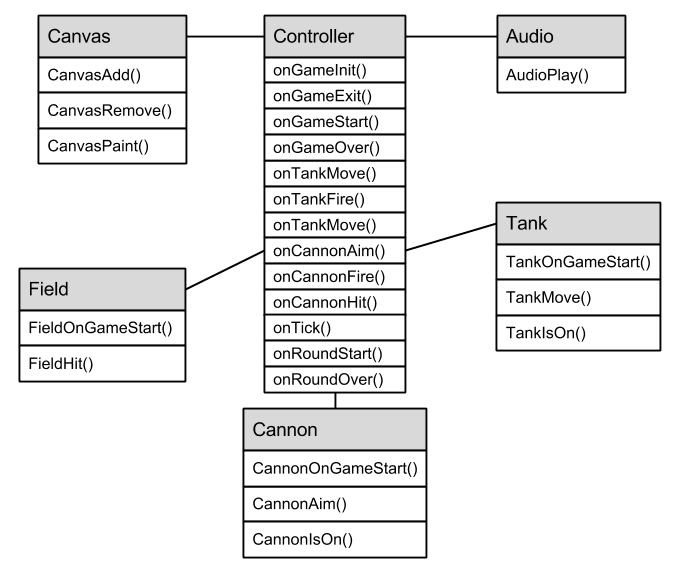
\includegraphics[width=350px]{graphics/game_UML.png}
  \caption{UML for the game design}
\end{figure}
